\documentclass[a4paper,12pt]{article}

\usepackage{geometry}       % Required for page layout.
\usepackage{hyperref}       % Required for hyperlinks.
\usepackage{graphicx}       % Required for figures.
\usepackage{subfig}         % Required for minipages.
\usepackage{float}          % Requried for optimal figure placement

\newgeometry{vmargin={25.4mm}, hmargin={27mm,27mm}}
\setlength\parindent{0pt}   % Disable paragraph indent.

\title{Studying the flow rate on a multi-lane using a cellular automata model}
\author{Erik Åsgrim}

\begin{document}
\maketitle

\section*{Introduction}
\subsection*{Background}
When planning efficient traffic infrastructure achieving efficient and safe traffic flow is of course very important.
A possible way of measuring how well traffic is flowing on a road is by studying the flow rate.
The flow rate on a road is defined as the sum of the velocities of the cars on the road divided by the length of the road.
In real life situations maximizing the flow rate could thus often be of interest. Another interesting metric to study is the fluctuations of the 
flow rate. If the flow rate does not fluctuate much the traffic flow is behaving in a stable way which could imply easier
driving conditions and a reduced risk of accidents.

In this report we will investigate how the flow rate behavior depends on the amount of lanes on the road and the car density by simulating
a highway using a cellular automata model.

\subsection*{Model description}
The model of the highway was implemented as a cellular automata on a road of some integer distance $L$ where each car on the road occupies $1$ length unit of the road. 
The road used periodic boundary conditions, meaning that the road does not have an end nor a beginning. The between the cars therefore also had to be calculated as periodic distances.
In order to make the dynamics of the simulation more realistic all cars were given personal maximum velocity $v_{i,max}$. The value of $v_{i, max}$ for each car was randomly generated 
as a rounded value taken from a Gaussian distribution around some mean value $\mu$, where $\mu$ would represent the speed limit on the road A Gaussian distribution of the values of $v_{i, max}$ thus
seems logical since in real life most cars drive at approximately the speed limit even though a few cars drive much faster or slower.

The rules for the cellular automata were performed in two different parts at each time step.
First, rules determining what lane changes are going to be performed are implemented. This was done by first calculating desired lane change of each car and then
performing the desired lane change only if the lane change can be performed safely.
Secondly, rules determining how the various cars are going to change their velocity are implemented.
Each rule was implemented simultaneously on each car before moving on to the next rule. This means that the ordering of the rules is very important, as latter rules can 'overrule' previous decisions.
In order to make the rules more compact we also introduce the following notation

\begin{itemize}
    \item $x_i$ is the position of the i:th car
    \item $v_i$ is the velocity of the i:th car
    \item $v_{i, max}$ is the maximum velocity of the i:th car.
    \item $v_{back}$ is the velocity to the next car backward in the \textbf{new lane} we would like to change to.
    \item $d_{forward}$ is the distance forward to the next car in the same lane we are currently in.
    \item $d_{forward, left}$ is the distance forward to the next car in the lane to the left.
    \item $d_{forward, right}$ is the distance forward to the next car in the lane to the right.
    \item $d_{backward}$ is the distance backward to next car in the \textbf{new lane} we would like to change to.
\end{itemize}

Using the above notation the rules of the cellular automata were implemented as follows:

\vspace{5pt}
\textbf{Lane changes}
\begin{enumerate}
    \item If $v_i<v_{i,max}$ and $d_{forward, left}\geq d_{forward}$ and there exists a lane to the left, desire a lane change from right to left
    \item If $d_{forward} > v_{i, max}$ and $d_{forward, right} > v_{i, max}$ and there exists a lane to the right, desire a lane change from left to right
    \item If $d_{forward, right} > d_{forward}$ and no previous lane change desire exists, desire a lane change from left to right with $5\%$ probability
    \item If $d_{backward} > v_{back}$ perform desired lane change (car behind should not need to brake because of lane change)
\end{enumerate}

\textbf{Velocity changes}
\begin{enumerate}
    \setcounter{enumi}{4}
    \item If $v_i<v_{i, max}$ increase velocity as $v_i \rightarrow v_i+1$ (try to accelerate to maximum velocity)
    \item If $v \geq d_{forward}$ decrease velocity as $v = d_{forward} - 1$ (avoid collisions)
    \item With some probability $p$ decrease velocity as $v_i=v_i-1$ (cars might brake randomly)
    \item Update position as $x_i(t+1) = x_i(t) + v_i$
\end{enumerate}

% Om det får plats, förklara logiken mer ingående av varje regel.
Most rules above are quite logical and result in a behavior of the cars that appears natural. Rule (3) might however need some
clarification. Without rule (3) mostly the left lane becomes occupied for higher car densities. In order to solve this rule (3) creates
a bias towards changing to the right lane which solves the problem.

% diskutera hur diskretiseringen av rum och tid kan påverka!!

\section*{Problem description}
The purpose of this report is to simulate a multi-lane highway and compare how the flow rate is affected by varying the number
of lanes at different car densities.
To do a statistical analysis of the result we would also like to examine the standard error of the flow rate and investigate whether the 
standard error of the flow rate varies depending on the car density and the number of lanes.

\section*{Method}
Initially the 

\section*{Results}
\begin{figure}[H]
    \centering
    \begin{minipage}{.5\textwidth}
        \centering
        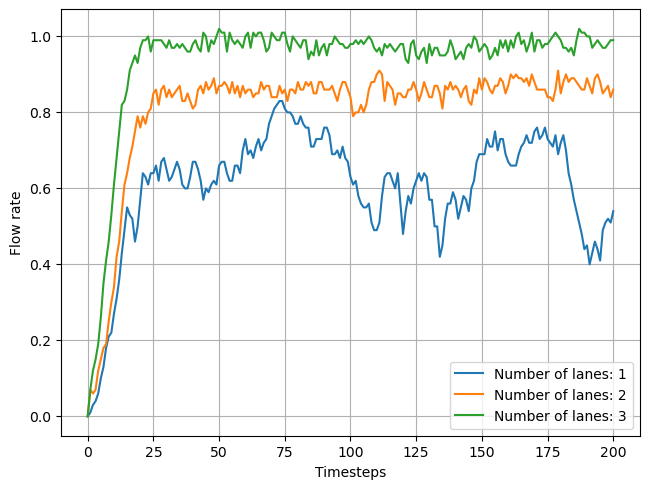
\includegraphics[scale=0.47]{Images/flowrate time 10 cars.png}
        \captionof*{figure}{a) 10 cars}
    \end{minipage}%
    \begin{minipage}{.5\textwidth}
        \centering
        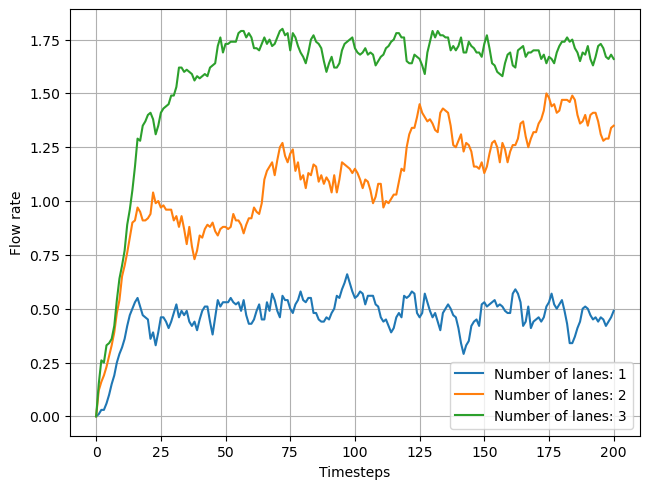
\includegraphics[scale=0.47]{Images/flowrate time 20 cars.png}
        \captionof*{figure}{b) 20 cars}
    \end{minipage}
    \centering
    \begin{minipage}{.5\textwidth}
        \centering
        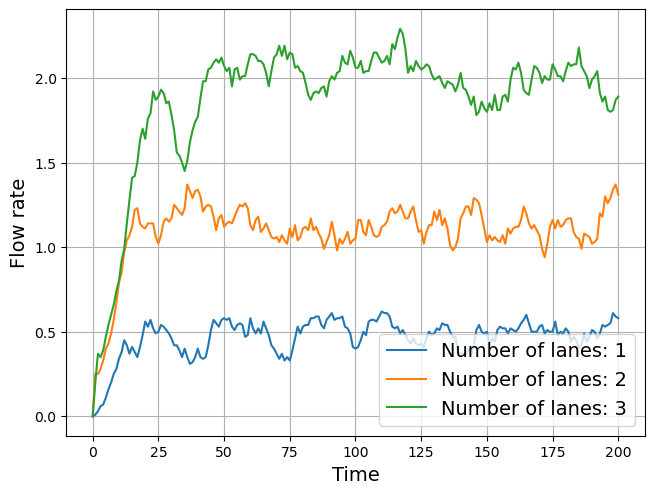
\includegraphics[scale=0.47]{Images/flowrate time 30 cars.png}
        \captionof*{figure}{c) 30 cars}
    \end{minipage}%
    \begin{minipage}{.5\textwidth}
        \centering
        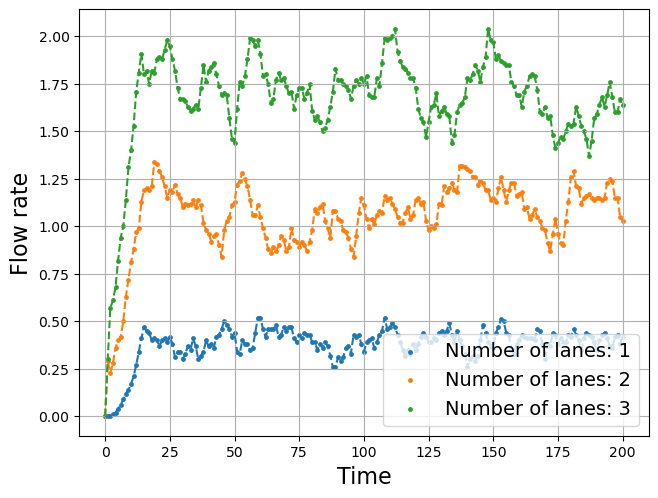
\includegraphics[scale=0.47]{Images/flowrate time 40 cars.png}
        \captionof*{figure}{d) 40 cars}
    \end{minipage}
    \caption{Flowrate plotted against time using different number of cars.}
    \label{flowrate}
\end{figure}

\begin{figure}[H]
    \centering
    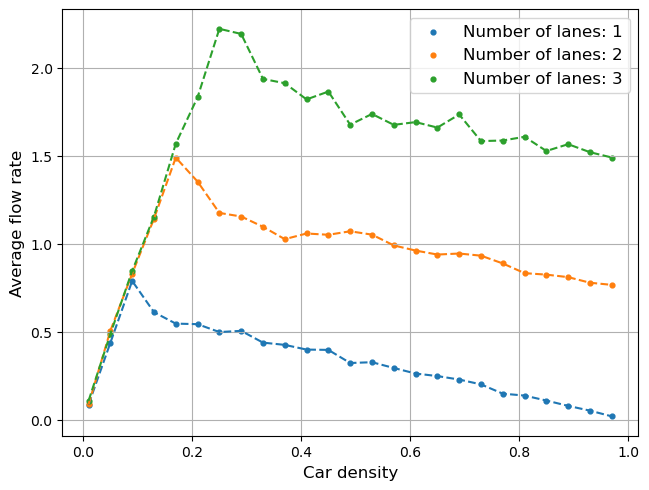
\includegraphics[scale=0.9]{Images/fundamental diagram.png}
    \caption{Average flow rate plotted against car density for different number of lanes.}
    \label{fundamental diagram}
\end{figure}

\subsection*{Statistical accuracy}
\begin{figure}[H]
    \centering
    \begin{minipage}{.5\textwidth}
        \centering
        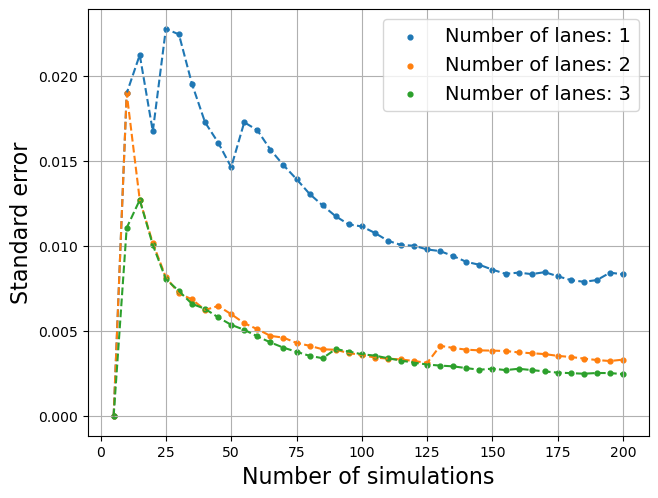
\includegraphics[scale=0.47]{Images/standard error 10 cars.png}
        \captionof*{figure}{a) 10 cars}
    \end{minipage}%
    \begin{minipage}{.5\textwidth}
        \centering
        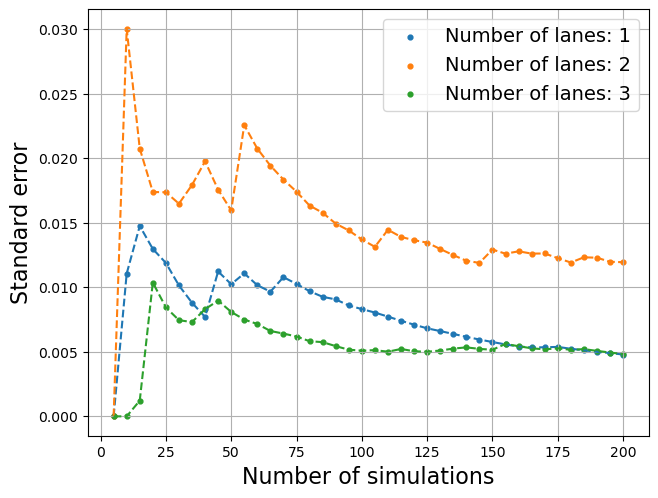
\includegraphics[scale=0.47]{Images/standard error 20 cars.png}
        \captionof*{figure}{b) 20 cars}
    \end{minipage}
    \centering
    \begin{minipage}{.5\textwidth}
        \centering
        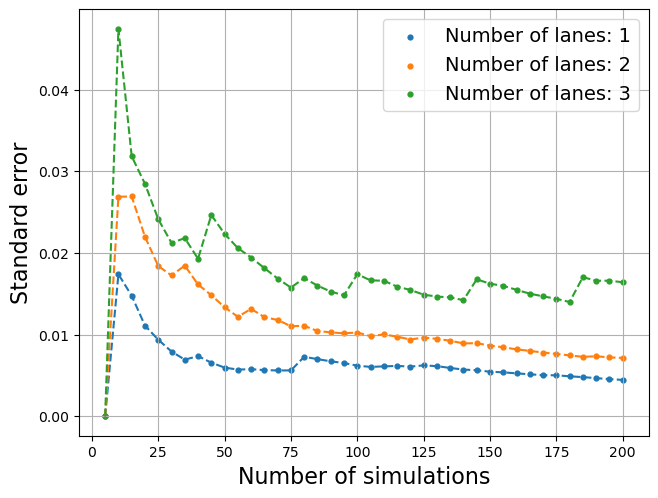
\includegraphics[scale=0.47]{Images/standard error 30 cars.png}
        \captionof*{figure}{c) 30 cars}
    \end{minipage}%
    \begin{minipage}{.5\textwidth}
        \centering
        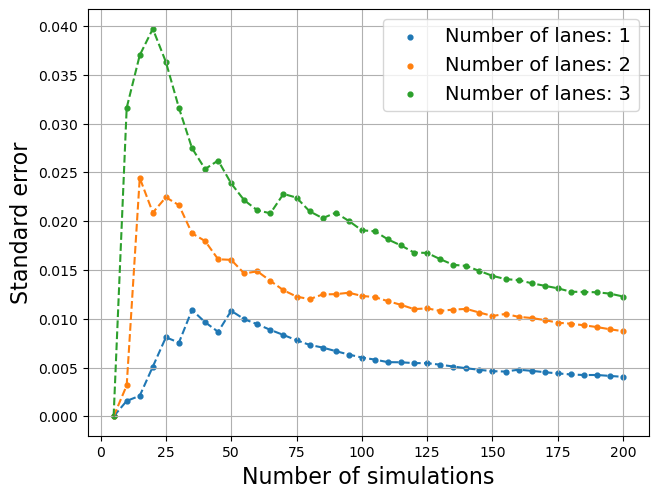
\includegraphics[scale=0.47]{Images/standard error 40 cars.png}
        \captionof*{figure}{d) 40 cars}
    \end{minipage}
    \caption{Standard error of average flowrate plotted against amount of simulations using different number of cars.}
    \label{flowrate}
\end{figure}

\begin{figure}[H]
    \centering
    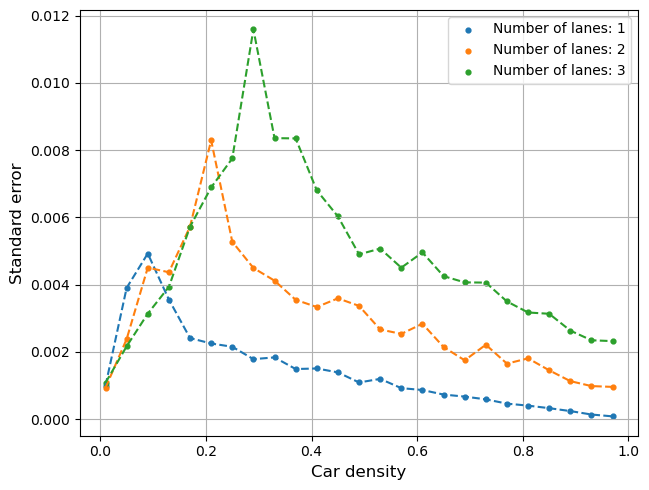
\includegraphics[scale=0.9]{Images/standard deviation.png}
    \caption{Standard error of average flow rate plotted against car density for different number of lanes.}
    \label{standard error}
\end{figure}


\section*{Discussion and analysis}
\subsection*{Model discussion}
% om det får plats, nämna omkörning på höger sida tillåtet??
In order to construct the above model several assumptions have been made. For example, the drivers have been assumed to be quite skilled
since a car will never perform a lane change if that means that a car behind will have to brake. In real life, this is of course true for some drivers 
but certainly not all.

Another assumption that has to be made since we are using the cellular automata is the fact that drivers only base their decisions on the current state. In other words, 
the drivers can never plan their driving in a way that skilled drivers would to in real life. For example ....

Another important aspect to mention are the possible consequences of using the period boundary conditions. When using period boundary conditions there is a risk
that a car might detect itself as the car in front. The car would then calculate the period distance to itself and adjust its speed accordingly. 
This is, of course, highly unrealistic and something we must be aware of when using the period boundary conditions. In order to reduce the risk of this happening
very short road lengths $L$ were avoided when running the simulation.
\end{document}